\documentclass[aspectratio=169]{beamer}

\usetheme{Boadilla}
\usecolortheme{seahorse}
\usepackage[T1]{fontenc}
\usepackage{lmodern}
\usepackage{booktabs}
\usepackage{pgfplots}
\pgfplotsset{compat=1.18}
\setbeamertemplate{navigation symbols}{}
\setlength{\emergencystretch}{2em}

\title{Python and Java Cache Experiments}
\subtitle{Project Checkpoint 2: LLC Capacity and Prefetching}
\author{Y Tagore Ravindra Sree}
\institute{CS683 Project}
\date{}

\begin{document}

\begin{frame}
  \titlepage
\end{frame}

\begin{frame}{What did I test?}
  \begin{block}{Two questions}
    \begin{enumerate}
      \item Does changing LLC size affect these program traces?
      \item Can simple prefetchers help with pointer chasing?
    \end{enumerate}
  \end{block}

  \vspace{0.4em}
  I tested five workloads in Python and Java. This checkpoint focuses on
  LLC capacity and the pointer-chase workload.
\end{frame}

\begin{frame}{How did I run the tests?}
  \begin{itemize}
    \item PIN captured instruction and memory-address traces.
    \item ChampSim replayed each trace; each captured trace has 1,000,000 instructions.
    \item The LLC sweep tested 0.5, 1, 2, 4, 8, and 16 MiB.
    \item LLC latency stayed at 20 cycles; other settings stayed at baseline.
    \item Pointer chasing compared no prefetching with \texttt{next\_line}
          and \texttt{ip\_stride} at L1D.
  \end{itemize}

  \begin{alertblock}{Important}
    These are simulator results for captured trace windows, not real
    processor timings.
  \end{alertblock}
\end{frame}

\begin{frame}{LLC size did not change the results}
  \begin{columns}[T,onlytextwidth]
    \column{0.63\textwidth}
      \centering
      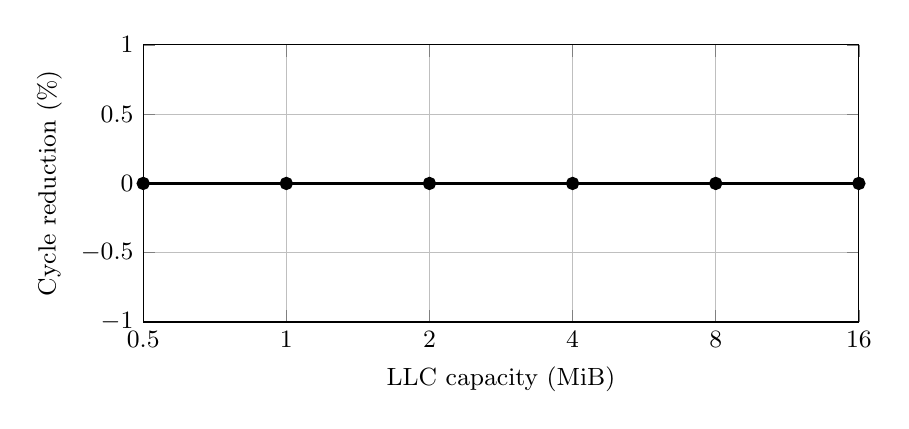
\begin{tikzpicture}
      \begin{axis}[
        width=0.88\linewidth,
        height=5.1cm,
        xmode=log,
        log basis x=2,
        xmin=0.5,
        xmax=16,
        xtick={0.5,1,2,4,8,16},
        xticklabels={$0.5$,$1$,$2$,$4$,$8$,$16$},
        xlabel={LLC capacity (MiB)},
        ylabel={Cycle reduction (\%)},
        ymin=-1,
        ymax=1,
        grid=major,
        tick label style={font=\small},
        label style={font=\small},
      ]
        \addplot[thick,mark=*] coordinates {
          (0.5,0) (1,0) (2,0) (4,0) (8,0) (16,0)
        };
      \end{axis}
      \end{tikzpicture}

    \column{0.35\textwidth}
      \begin{itemize}
        \item All ten workload traces had the same cycle count at every tested size.
        \item Miss counts also stayed the same.
        \item No capacity point showed a measurable improvement.
      \end{itemize}
  \end{columns}
\end{frame}

\begin{frame}{Pointer-chase results}
  \scriptsize
  \centering
  \resizebox{\textwidth}{!}{%
  \begin{tabular}{llrr}
    \toprule
    Runtime & L1D prefetcher & Cycles & Change \\
    \midrule
    Python & None & 908,178 & -- \\
    Python & Next-line & 809,460 & 10.87\% fewer \\
    Python & IP-stride & 870,068 & 4.20\% fewer \\
    \midrule
    Java & None & 1,048,083 & -- \\
    Java & Next-line & 1,070,226 & 2.11\% more \\
    Java & IP-stride & 1,048,085 & About the same \\
    \bottomrule
  \end{tabular}
  }

  \vspace{0.7em}
  \begin{block}{What stands out?}
    Both prefetchers helped the Python trace. Neither helped the Java trace.
  \end{block}
\end{frame}

\begin{frame}{What might explain this?}
  \begin{itemize}
    \item Python memory-wait share fell from 47.96\% to 41.29\% with next-line
          prefetching.
    \item Java memory-wait share stayed around 75.46\%.
    \item Only a small fraction of issued prefetches were useful, especially
          for Java.
    \item The flat LLC results could mean little reuse in the captured window,
          or a working set larger than the tested range.
  \end{itemize}

  \begin{alertblock}{Careful interpretation}
    The Python result is worth testing again, but it does not mean that
    prefetching will help all Python programs.
  \end{alertblock}
\end{frame}

\begin{frame}{Limits of this experiment}
  \begin{itemize}
    \item One trace window was tested for each workload; there were no repeat runs.
    \item ChampSim replays traces. It does not measure application run time on
          a real CPU.
    \item Interpreter and JVM instructions are part of the traces.
    \item Python and Java use different data layouts, so this is not a
          language-wide comparison.
    \item LLC latency stayed fixed while capacity changed.
  \end{itemize}
\end{frame}

\begin{frame}{Takeaway and next step}
  \begin{block}{Main takeaway}
    LLC sizes from 0.5 to 16 MiB made no measurable difference in these
    workloads. The Python pointer-chase trace improved with the tested
    prefetchers; the Java trace did not.
  \end{block}

  \begin{block}{What I would test next}
    Use longer and repeated trace windows, and include a workload with known
    reuse in the LLC.
  \end{block}

  \vfill
  \centering
  \small Results are clues about these traces, not a general ranking of Python
  and Java.
\end{frame}

\end{document}
